\documentclass[a4paper, 12pt]{article}

\usepackage{float}
\usepackage[margin=1in,top=2cm, bottom=2cm]{geometry}

\usepackage[T1]{fontenc}
\usepackage[utf8]{inputenc}

\usepackage[mono=false]{libertine}
\usepackage[libertine]{newtxmath}
\usepackage[scaled=0.97]{zi4}
\usepackage{csquotes}

\usepackage[english,portuguese]{babel}
\usepackage[backend=biber]{biblatex}

\usepackage[dvipsnames]{xcolor}
\usepackage{graphicx}

% Skip paragraphs instead of indenting
\usepackage{parskip}

\usepackage{url}
\usepackage{hyperref}

\usepackage{fancyhdr}
\usepackage{sectsty}
\usepackage{secdot}

\usepackage{caption}
\usepackage{subcaption}
\usepackage{biblatex}
\usepackage{float}

\usepackage{enumitem}
\usepackage{multicol}

\usepackage{fontawesome5}

\bibliography{references.bib}

\captionsetup[subfigure]{labelformat=empty}
\captionsetup{justification=centering}

\newcommand{\email}[1]{\textcolor{RedOrange}{\faIcon{envelope}} \large{\href{mailto:#1}{#1}}}
\newcommand{\studentID}[1]{\textcolor{BlueGreen}{\faIcon{id-card}} \large{#1}}

\renewcommand{\headrulewidth}{0.2mm}
\renewcommand{\headruleskip}{0.8mm}

\sectionfont{\sffamily\LARGE}
\subsectionfont{\sffamily\Large}
\subsubsectionfont{\sffamily\large}

\sectiondot{section}
\sectiondot{subsection}
\sectiondot{subsubsection}

\sectionpunct{section}{. }
\sectionpunct{subsection}{. }
\sectionpunct{subsubsection}{. }

\setlength{\headheight}{20pt}

\fancypagestyle{Multimedia}{%
	\fancyhf{}
	\fancyhead[R]{
		\ifodd\value{page}
			\sffamily Multimédia --- 2022/2023%
		\else
			\sffamily Relatório
		\fi
	}
	%\fancyhead[L]{
	%	  \includegraphics[scale=0.01,keepaspectratio]{resources/titlepage/fpce-cpsc-uc-logo.png}
	%	\sffamily{Multimedia}
	%}
	\fancyfoot[C]{\thepage}
}
\pagestyle{Multimedia}


\begin{document}

\begin{titlepage}
	\centering

	\begin{figure}[H]
		\centering
		
\includegraphics[scale=0.15]{resources/uc.png}
		%\hfill
	\end{figure}

	\vspace{5cm}
	\Huge{\sffamily \textbf {Compressão de imagem}} \\
	\vspace{0.2cm}
	\LARGE{\sffamily Multimédia} \\

	%\begin{figure}[H]
	%	\centering
	%	
\includegraphics[width=\textwidth,height=\textheight,keepaspectratio]{resources/fctuc.png}
	%	%\hfill
	%\end{figure}
 
	\vspace{1cm}
	\Large{\sffamily Licenciatura em Engenharia Informática} \\
	\Large{\sffamily 2022/2023} \\
	\vspace{0.4cm}
	\large{\sffamily\today}
\end{titlepage}

\section*{Autores}

    \begin{itemize}[label={},leftmargin=*]
	\item \textbf{João Moreira}
	      \subitem {\email{joaomoreira@student.dei.uc.pt}}
	      \subitem {\studentID{2020230563}}
	\item	\textbf{Rodrigo Figueiredo}
	      \subitem {\email{rfigueiredo@student.dei.uc.pt}}
	      \subitem {\studentID{2020236687}}
	\item	\textbf{Tomás Pinto}
	      \subitem {\email{tomaspinto@student.dei.uc.pt}}
	      \subitem {\studentID{2020224069}}
       
\end{itemize}

\pagebreak

\renewcommand*\contentsname{Índice}
\tableofcontents
\pagebreak

\section{Introdução}
Compressão de dados de imagem é a técnica de reduzir o tamanho original de uma imagem de forma a manter a sua qualidade.

Ao contrário do que foi desenvolvido em Teoria da Informação (compressão de dados sem perda),
neste trabalho pretende-se explorar a compressão com perda de informação.
Neste tipo de algoritmo, tentamos reduzir o tamanho original da imagem com a perda de parte da informação inicial.

Sendo assim, o objetivo principal é explorar a informação pouco relevante visualmente para o ser Humano, de forma que
ao elimina-la seja impercetível ao olho humano.
O codec que iremos usar é o JPEG.


\printbibliography[heading=none]

\pagebreak
\section{Compressão de Imagem Com um Editor Auxiliar}
    Começámos por comprimir as 3 imagens fornecidas em formato bmp para o formato jpeg nas qualidades alta
    (75\%), média (50\%) e baixa (25\%) utilizando o GIMP. Os resultados obtidos são apresentados de seguida. 
    
    \subsection{Resultados}
        \begin{table}[h!]
            \centering
            \addtolength\tabcolsep{20pt}
            \begin{tabular}{||c | c c c||} 
                \hline
                Compress & Barn\_Mountains & Logo & Peppers \\ 
                \hline\hline
                Original & 348 & 411 & 576  \\ 
                High & 33 & 9.4 & 30.5  \\
                Medium & 21.5 & 7.6 & 20.3  \\
                Low & 13.5 & 6.2 & 13.3  \\
                \hline
            \end{tabular}
            \caption{\label{demo-table} Tamanho final das imagens em Kb.}
        \end{table}
        \begin{table}[h!]
            \centering
            \addtolength\tabcolsep{20pt}
            \begin{tabular}{||c | c c c||} 
                \hline
                Compress & Barn\_Mountains & Logo & Peppers \\ 
                \hline\hline
                High   & 10:1 & 44:1 & 19:1  \\
                Medium & 16:1 & 54:1 & 28:1  \\
                Low    & 26:1 & 66:1 & 43:1  \\
                \hline
            \end{tabular}
            \caption{\label{demo-table} Racio das compressões por imagem.}
        \end{table}
    \subsection{Analise de Resultados}
        Como era esperado, os resultados mostram uma diminuição de tamanho dos ficheiros quando as imagens 
        originais são comprimidas. Podemos verificar que quanto menor é a qualidade menor é o tamanho do
        ficheiro também.   
        
        Algo interessante de observar é que conseguimos comprimir mais de dez vezes o ficheiro original e 
        manter uma qualidade alta.

        Ao olhar para as imagens de \textbf{qualidade alta} é notório alguma perda de qualidade. 
        As principais zonas onde se nota maior perda de qualidade é nas transições abruptas de cor.
        Por exemplo, na imagem \emph{logo.bmp} observa-se grandes perdas junto às transições de cores,
        não se notando perdas nas partes de cores constantes.

        Este comportamento é característico do JPEG, visto que ele explora as limitações do olho Humano
        e acaba por perder alguma sensibilidade nas zonas de transições abruptas.

        Sendo assim, concluímos que o JPEG tem uma maior compressão para imagens com transições abruptas
        de cor (o que gera mais ruído/distorção) e trás mais qualidade para imagens com transições suaves
        de cor.
          

\pagebreak
\section{Modelo YCbCr vs Modelo RGB}
    Foi feita a conversão das imagens do modelo RGB inicial para o modelo YCbCr. 
    
    O modelo RGB possui redundância da luminância nos 3 canais. Esta conversão é importante pois este
    modelo permite-nos separar as componente da luminância (canal Y)
    e da crominância (canais Cb e Cr), que se encontram fundidas no modelo RGB. 
    
    Como a visão humana é mais sensível à luminância, o JPEG pode tirar proveito disso para comprimir mais
    nas componentes Cb e Cr que irão influenciar muito menos a qualidade da imagem final a olho nu
    comparativamente à componente Y.
    
    \subsection{Resultados}
        \begin{multicols}{3}
            \begin{figure}[H]
                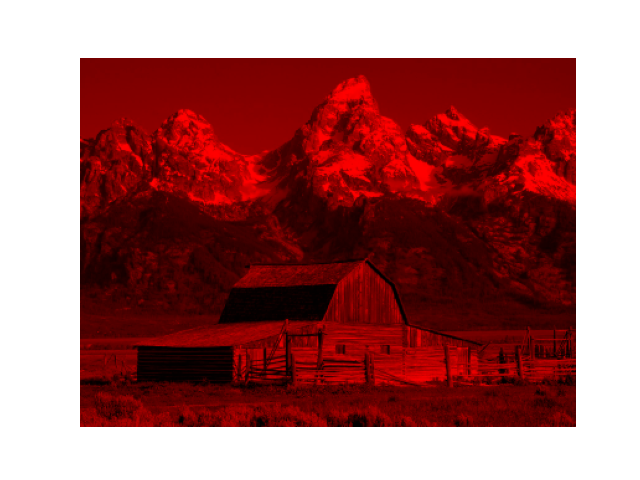
\includegraphics[width=\linewidth]{resources/Exercicio4/R.png}
                \caption{\label{fig:my_label} Canal R}
            \end{figure}
            \begin{figure}[H]
                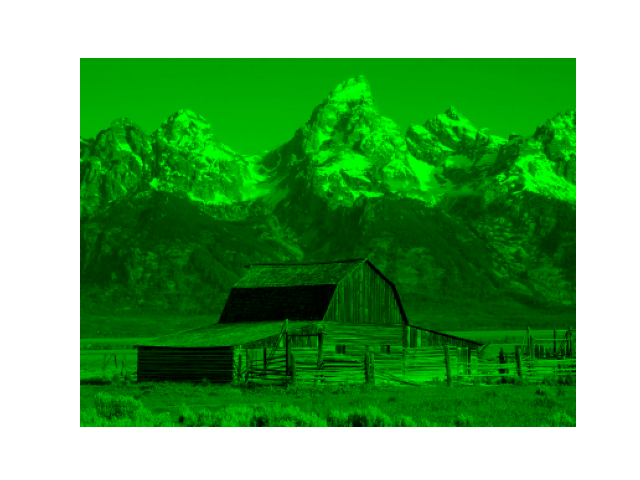
\includegraphics[width=\linewidth]{resources/Exercicio4/G.png}
                \caption{\label{fig:my_label} Canal G}
            \end{figure}
            \begin{figure}[H]
                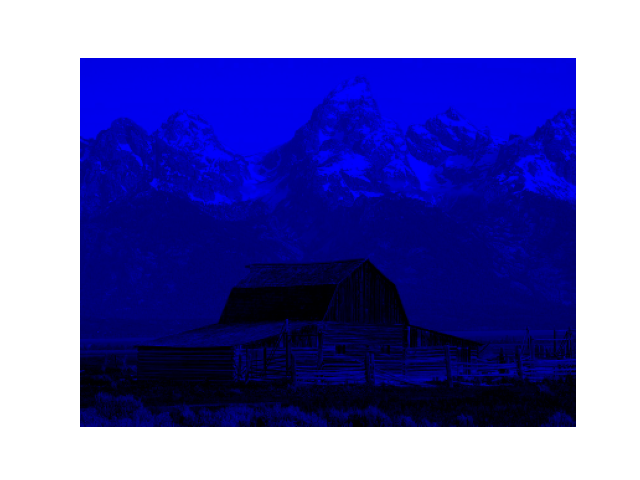
\includegraphics[width=\linewidth]{resources/Exercicio4/B.png}
                \caption{\label{fig:my_label} Canal B}
            \end{figure}
        \end{multicols}
        Podemos reparar que nas imagens acima, apesar dos três canais R, G e B  conterem luminância, o nível de detalhe não é igual em todos. Isto é devido ao facto do olho humano ser mais sensível às tonalidades verdes, de seguida vermelhas e por ultimo azuis, coincidente com a ordem decrescente de detalhe das três imagens.   
        
        \begin{multicols}{3}
            \begin{figure}[H]
                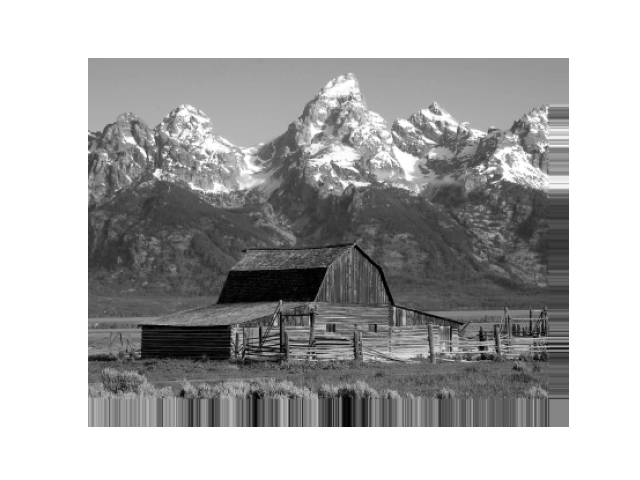
\includegraphics[width=\linewidth]{resources/Exercicio4/Y.png}
                \caption{\label{fig:my_label} Canal Y}
            \end{figure}
            \begin{figure}[H]
                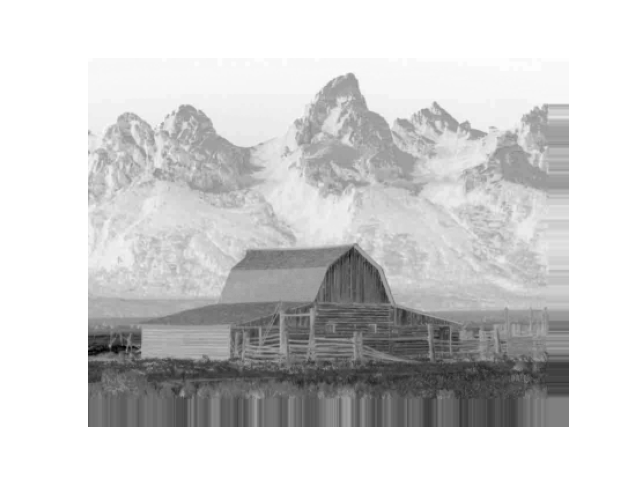
\includegraphics[width=\linewidth]{resources/Exercicio4/CB.png}
                \caption{\label{fig:my_label} Canal CB}
            \end{figure}
            \begin{figure}[H]
                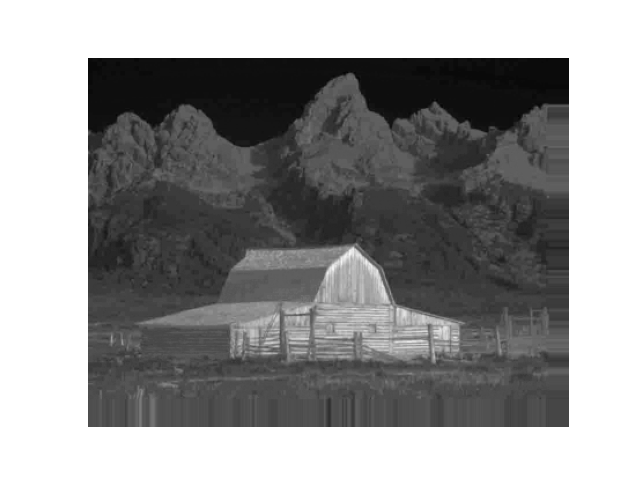
\includegraphics[width=\linewidth]{resources/Exercicio4/CR.png}
                \caption{\label{fig:my_label} Canal CR}
            \end{figure}
        \end{multicols}

        Como é possível ver pelas imagens, o canal Y (canal da luminância) apresenta mais detalhe do que
        os canais Cb e Cr (canais da crominância). Isto deve-se não à perda de qualidade, mas sim ao facto
        de o olho humano ter maior sensibilidade à luminância do que a crominância.

        Sendo assim, iremos ver ao longo do trabalho como o JPEG usa os canais Cb e Cr a seu favor.\\[8pt]
        
        \textit{Nota: Para melhor visualização as imagens relativas aos canais Y, Cb e Cr são aplicadas um \emph{colormap}
        de tons de cinza.}
        
\pagebreak
\section{Sub-Amostragem}
    Na fase da sub-amostragem, \emph{downsampling}, é reduzida a quantidade de dados nos canais relativos à cor (Cb
    e Cr) com o objetivo de melhorar a compressão, o que resulta numa resolução espacial menor nas imagens,
    pelo que não há alterações no canal Y. 
    
    Como explicado anteriormente, o olho humano é menos sensível à crominância e a redução de informação
    pode ser feita sem comprometer significativamente a qualidade da imagem final.

    Sendo assim, de forma a diminuir a informação podemos remover parte dela:
    \begin{itemize}
        \item Sub-amostragem $4:2:2$ a imagem ficará reduzida horizontalmente, com metade das 
    colunas.
        \item Sub-amostragem $4:2:0$ a imagem ficará reduzida verticalmente e horizontalmente, 
    com metade das colunas e linhas.
    \end{itemize}
    
    Nesta redução foi aplicada uma interpolação cúbica (opção do grupo de trabalho).

    %\subsection{Resultados}
        \begin{multicols}{2}
            \begin{figure}[H]
                \centering
                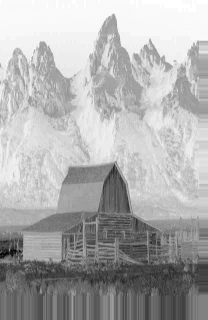
\includegraphics[scale=1]{resources/Sampling/CB_422.png}
                \caption{\label{fig:my_label} Sub-amostragem canal CB 4:2:2}
            \end{figure}
            \begin{figure}[H]
                \centering
                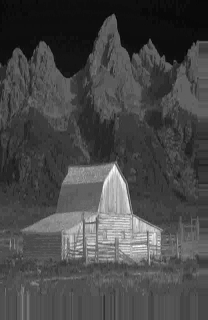
\includegraphics[scale=1]{resources/Sampling/CR_422.png}
                \caption{\label{fig:my_label} Sub-amostragem canal CR 4:2:2}
            \end{figure}
        \end{multicols}

        \vspace{1cm}

        \begin{multicols}{2}
            \begin{figure}[H]
                \centering
                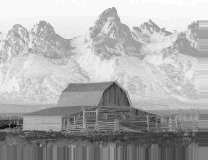
\includegraphics[scale=1]{resources/Sampling/CB_420.png}
                \caption{\label{fig:my_label} Sub-amostragem canal CB 4:2:0}
            \end{figure}
            \begin{figure}[H]
                \centering
                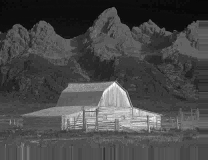
\includegraphics[scale=1]{resources/Sampling/CR_420.png}
                \caption{\label{fig:my_label} Sub-amostragem canal CR 4:2:0}
            \end{figure}
        \end{multicols}
        
    \subsection{Resultados}
        \begin{table}[H]
            \centering
            \addtolength\tabcolsep{20pt}
            \begin{tabular}{||c | c ||} 
                \hline
                Imagens & Tamanho \\
                \hline\hline
                Cb      & 122 \\
                Cr      & 112 \\
                Cb\_422 & 57  \\
                Cr\_422 & 54  \\
                Cb\_420 & 34  \\
                Cr\_420 & 32  \\ 
                \hline
            \end{tabular}
            \caption{\label{demo-table} Tamanho final das sub-amostragens em Kb.}
        \end{table}
        
        \begin{table}[H]
            \centering
            \addtolength\tabcolsep{20pt}
            \begin{tabular}{||c | c ||} 
                \hline
                Imagens           & Taxa de Compressão \\
                \hline\hline
                Cb\_422 & $2 : 1$ \\
                Cr\_422 & $2  : 1$  \\
                Cb\_420 & $4  : 1$  \\
                Cr\_420 & $4  : 1$  \\ 
                \hline
            \end{tabular}
            \caption{\label{demo-table} Taxa de compressão das sub-amostragens.}
        \end{table}
        
    \subsection{Análise de resultados}
        Como era esperado, para fatores $4:2:2$ o tamanho das imagens diminui para metade e fatores $4:2:0$
        reduziu para um quarto do tamanho original.
        É possível observar também que os detalhes mantém-se apesar de a informação ter diminuído.

        Apesar de o fator $4:2:0$ apresentar uma maior compressão face o fator $4:2:2$, em contra partida
        é o que apresenta maior destrutividade.

        Para as outras imagens, vai-se observar o mesmo comportamento.

        %\textit{Nota: No fator $4:2:0$ estávamos à espera de comprimir quatro vezes a imagem visto que diminuimos
        %a dimensão para tal.
        %No entanto, não é o que observamos. Dois motivos pelo qual isto acontece pode ser o facto de usarmos
        %uma interpolação cúbica e o formato que guardamos a imagem final, \emph{png}.}
        

\pagebreak        
\section{Transformada de Cosseno Discreto}
    A DCT permite-nos converter um sinal num espectro de frequências. Desta forma, em imagens podemos
    converter o valor de cada píxel para o domínio da frequência, o que nos permite ter uma análise das
    frequências que estão a ser usadas na imagem e estabelecer uma relação com aquelas que ao olho Humano
    não é tão sensível.

    Visto que a DFT resulta em números imaginários e tem um padrão repetitivo, seria necessário o
    dobro da memória face à DCT. Sendo assim, é mais vantajoso usar a DCT.
    
    \subsection{Aplicação da DCT no Canal Completo}        
        \begin{figure}[H]
            \ContinuedFloat
            \begin{subfigure}{0.3\textwidth}
                \centering
                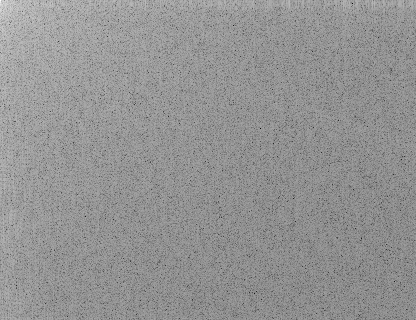
\includegraphics[scale=0.5]{resources/DCT/Ydct.png}
                \caption{ Canal Y.}
            \end{subfigure}
            \hfill
            \begin{subfigure}{0.3\textwidth}
                \centering 
                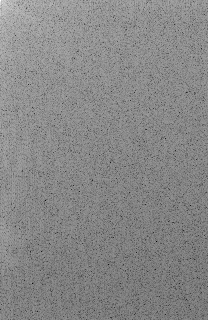
\includegraphics[scale=0.5]{resources/DCT/CBdct.png}
                \caption{ Canal Cb.}
            \end{subfigure}
            \hfill
            \begin{subfigure}{0.3\textwidth}
                \centering
                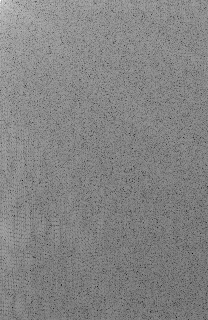
\includegraphics[scale=0.5]{resources/DCT/CRdct.png} 
                \caption{ Canal Cr.}
            \end{subfigure}
            \caption{ DCT da imagem Barn\_Mountains.}
            \label{fig:my_label}
        \end{figure}

        Como vemos na \emph{Figura 11}, observamos que os coeficientes DC e AC mais
        altos
        concentram-se no canto superior esquerdo, ou seja, aquele ponto cintilante é
        representativo de alta energia para as baixas frequências e os tons mais escuros 
        representam baixa energia nas altas frequências.
        Logo, significa que estamos perante uma imagem de transições suaves, o que se comprova, pois
        este espectro pertence à \emph{Figura Barn\_Mountains}.

        Visto que na gama de altas frequências da \emph{Figura Barn\_Mountains} apresenta baixa energia,
        ela irá comprimir menos do que a \emph{Figura Logo}, que em contra partida apresenta alta energia ao
        longo do espectro de frequências.
        Pela mesma razão, a \emph{Figura Barn\_Mountains} irá apresentar menos ruído do que a 
        \emph{Figura Logo}.
        \begin{figure}[H]
            \begin{subfigure}{0.3\textwidth}
                \centering
                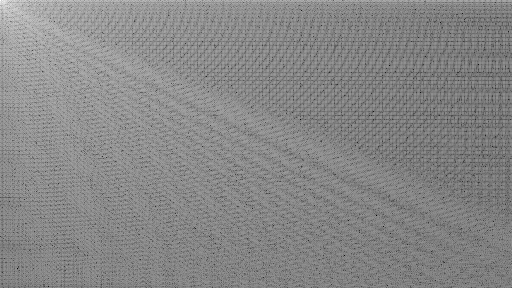
\includegraphics[width=\textwidth]{resources/DCT/Ydct_logo.png}
                \caption{ Canal Y.}
            \end{subfigure}
            \hfill
            \begin{subfigure}{0.3\textwidth}
                \centering 
                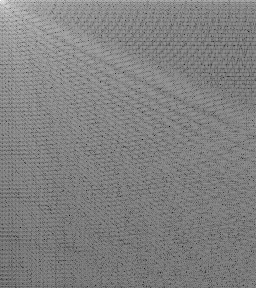
\includegraphics[scale=0.5]{resources/DCT/CBdct_logo.png}
                \caption{ Canal Cb.}
            \end{subfigure}
            \hfill
            \begin{subfigure}{0.3\textwidth}
                \centering
                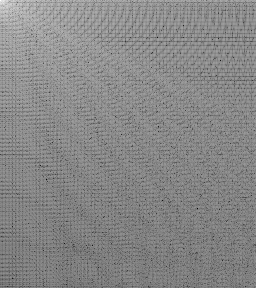
\includegraphics[scale=0.5]{resources/DCT/CRdct_logo.png} 
                \caption{ Canal Cr.}
            \end{subfigure}
            \caption{ DCT da imagem Logo.}
            \label{fig:my_label}
        \end{figure}

        Ao analisar a \emph{Figura 12} vemos que existe uma variação de energia ao 
        longo das altas e baixas frequências, o que significa que esta imagem apresenta
        simultaneamente transições suaves e abruptas. Neste exemplo, trata-se da 
        \emph{Figura logo}.

        Espectros de altas frequências com baixa energia têm tendência a comprimir e destruir mais,
        em relação a espectros de baixas frequências.

    \subsection{Aplicação da DCT em Blocos 8x8}
        \begin{figure}[H]
            \begin{subfigure}{0.3\textwidth}
                \centering
                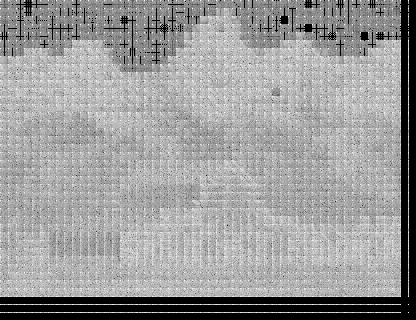
\includegraphics[scale=0.5]{resources/DCT/Ydct8.png}
                \caption{ Canal Y.}
            \end{subfigure}
            \hfill
            \begin{subfigure}{0.3\textwidth}
                \centering 
                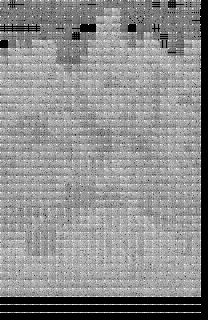
\includegraphics[scale=0.5]{resources/DCT/CBdct8.png}
                \caption{ Canal Cb.}
            \end{subfigure}
            \hfill
            \begin{subfigure}{0.3\textwidth}
                \centering
                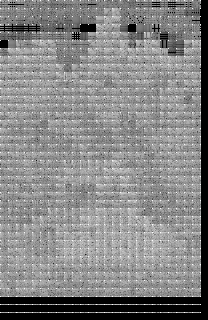
\includegraphics[scale=0.5]{resources/DCT/CRdct8.png}
                \caption{ Canal Cr.}
            \end{subfigure}
            \caption{\label{fig:my_label} DCT da imagem Barn\_Mountains em blocos 8x8.}
        \end{figure}

        Como é visível nas imagens acima, quase que é possível reconhecer a imagem inicial.
        A primeira observação a notar é que o canal Y tem mais detalhes. Um motivo plausível para isso 
        acontecer é o facto de os canais Cb e Cr terem sofrido destruição na sub-amostragem e o canal Y
        permanecer \emph{"virgem"}.

        Isto acontece, porque ao limitar o nosso sinal a blocos de 8x8 a probabilidade de ocorrer transições
        de cores abruptas diminui, no que resulta um sinal de transições de cores suaves.

        A aplicação da DCT em blocos 8x8 tem um maior potencial de compressão em relação à imagem inteira
        pois as altas frequências têm maior probabilidade de terem baixa energia, ou seja, existirá
        um maior número de coeficientes AC nulos ou próximos de zero.\\

        \begin{figure}[H]
            \begin{subfigure}{0.3\textwidth}
                \centering
                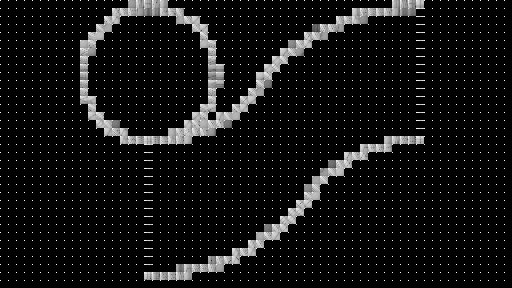
\includegraphics[width=\textwidth]{resources/DCT/Ydct8_logo.png}
                \caption{ Canal Y.}
            \end{subfigure}
            \hfill
            \begin{subfigure}{0.3\textwidth}
                \centering 
                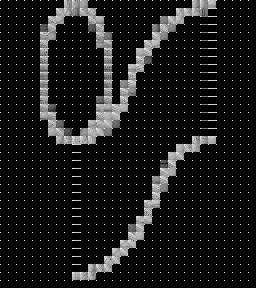
\includegraphics[scale=0.5]{resources/DCT/CBdct8_logo.png}
                \caption{ Canal Cb.}
            \end{subfigure}
            \hfill
            \begin{subfigure}{0.3\textwidth}
                \centering
                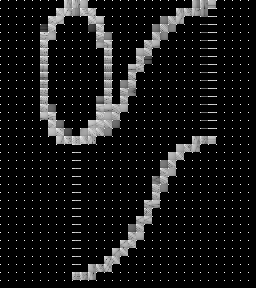
\includegraphics[scale=0.5]{resources/DCT/CRdct8_logo.png}
                \caption{ Canal Cr.}
            \end{subfigure}
            \caption{\label{fig:my_label} DCT da imagem Barn\_Mountains em blocos 8x8.}
        \end{figure}

        Nas figuras que antecedem, facilmente verificamos o que foi descrito anteriormente:
        como existe poucas zonas de transições, a maior parte dos coeficientes AC estão a zero e têm um 
        maior potencial de compressão.

        \subsection{Aplicação da DCT em Blocos 64x64}
        \begin{figure}[H]
            \begin{subfigure}{0.3\textwidth}
                \centering
                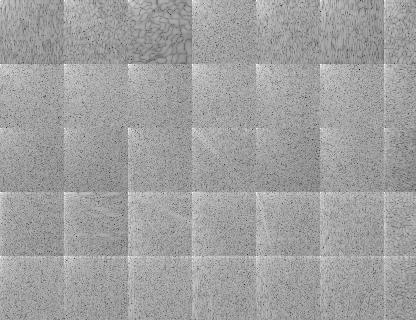
\includegraphics[scale=0.5]{resources/DCT/Ydct64.png}
                \caption{ DCT do canal Y em blocos 64x64}
            \end{subfigure}
            \hfill
            \begin{subfigure}{0.3\textwidth}
                \centering 
                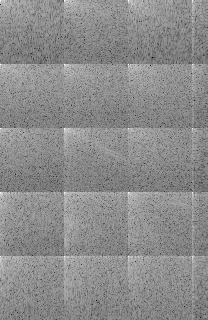
\includegraphics[scale=0.5]{resources/DCT/CBdct64.png}
                \caption{ DCT do canal Cb em blocos 64x64}
            \end{subfigure}
            \hfill
            \begin{subfigure}{0.3\textwidth}
                \centering
                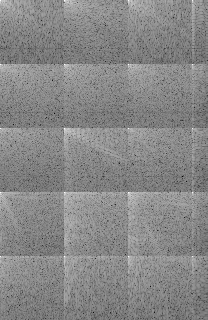
\includegraphics[scale=0.5]{resources/DCT/CRdct64.png}
                \caption{ DCT do canal Cr em blocos 64x64}
            \end{subfigure}
            \caption{\label{fig:my_label} DCT da imagem Barn\_Mountains em blocos 64x64.}
        \end{figure}

        Como podemos observar aplicar a DCT em blocos de 64x64 deixa o canal ainda muito homogéneo.
        Com esta estratégia iremos ter melhor compressão do que com o canal inteiro, mas se aplicado
        com blocos de 8x8 teremos resultados muito melhores.


\pagebreak
\section{Quantização}
    O olho humano não tem tanta sensibilidade para distinguir componentes de altas frequências
    (estas frequências correspondes às transições abruptas).

    No processo de quantização divide-se as frequências por um valor de quantização já
    pre-determinado, aliado a um fator de qualidade.
    Isso permite-nos remover facilmente as altas frequências da imagem (já calculadas pela DCT), 
    pois são menos importantes para o olho humano.
        \begin{figure}[H]
            \begin{subfigure}{0.3\textwidth}
                \centering
                \includegraphics[scale=0.5]{resources/Quantization/YQuantization10.png}
                \caption{ Canal Y.}
            \end{subfigure}
            \hfill
            \begin{subfigure}{0.3\textwidth}
                \centering 
                \includegraphics[scale=0.5]{resources/Quantization/CBQuantization10.png}
                \caption{ Canal Cb.}
            \end{subfigure}
            \hfill
            \begin{subfigure}{0.3\textwidth}
                \centering
                \includegraphics[scale=0.5]{resources/Quantization/CRQuantization10.png} 
                \caption{ Canal Cr.}
            \end{subfigure}
            \caption{\label{fig:my_label} Quantização da imagem Barn\_Mountains qualidade 10.}
        \end{figure}
        
        \vspace{0.5cm}
    
        \begin{figure}[H]
            \begin{subfigure}{0.3\textwidth}
                \centering
                \includegraphics[scale=0.5]{resources/Quantization/YQuantization25.png}
                \caption{ Canal Y.}
            \end{subfigure}
            \hfill
            \begin{subfigure}{0.3\textwidth}
                \centering 
                \includegraphics[scale=0.5]{resources/Quantization/CBQuantization25.png}
                \caption{ Canal Cb.}
            \end{subfigure}
            \hfill
            \begin{subfigure}{0.3\textwidth}
                \centering
                \includegraphics[scale=0.5]{resources/Quantization/CRQuantization25.png} 
                \caption{ Canal Cr.}
            \end{subfigure}
            \caption{\label{fig:my_label} Quantização da imagem Barn\_Mountains qualidade 25.}
        \end{figure}
        
        \vspace{0.5cm}
    
        \begin{figure}[H]
            \begin{subfigure}{0.3\textwidth}
                \centering
                \includegraphics[scale=0.5]{resources/Quantization/YQuantization50.png}
                \caption{ Canal Y.}
            \end{subfigure}
            \hfill
            \begin{subfigure}{0.3\textwidth}
                \centering 
                \includegraphics[scale=0.5]{resources/Quantization/CBQuantization50.png}
                \caption{ Canal Cb.}
            \end{subfigure}
            \hfill
            \begin{subfigure}{0.3\textwidth}
                \centering
                \includegraphics[scale=0.5]{resources/Quantization/CRQuantization50.png} 
                \caption{ Canal Cr.}
            \end{subfigure}
            \caption{\label{fig:my_label} Quantização da imagem Barn\_Mountains qualidade 50.}
        \end{figure}
            
        \vspace{0.5cm}
        
        \begin{figure}[H]
            \begin{subfigure}{0.3\textwidth}
                \centering
                \includegraphics[width=\linewidth]{resources/Quantization/YQuantization75.png}
                \caption{ Canal Y.}
            \end{subfigure}
            \hfill
            \begin{subfigure}{0.3\textwidth}
                \centering 
                \includegraphics[scale=0.5]{resources/Quantization/CBQuantization75.png}
                \caption{ Canal Cb.}
            \end{subfigure}
            \hfill
            \begin{subfigure}{0.3\textwidth}
                \centering
                \includegraphics[scale=0.5]{resources/Quantization/CRQuantization75.png} 
                \caption{ Canal Cr.}
            \end{subfigure}
            \caption{\label{fig:my_label} Quantização da imagem Barn\_Mountains qualidade 75.}
        \end{figure}
        
        \vspace{0.5cm}

        \begin{figure}[H]
            \begin{subfigure}{0.3\textwidth}
                \centering
                \includegraphics[scale=0.5]{resources/Quantization/YQuantization100.png}
                \caption{ Canal Y.}
            \end{subfigure}
            \hfill
            \begin{subfigure}{0.3\textwidth}
                \centering 
                \includegraphics[scale=0.5]{resources/Quantization/CBQuantization100.png}
                \caption{ Canal Cb.}
            \end{subfigure}
            \hfill
            \begin{subfigure}{0.3\textwidth}
                \centering
                \includegraphics[scale=0.5]{resources/Quantization/CRQuantization100.png} 
                \caption{ Canal Cr.}
            \end{subfigure}
            \caption{\label{fig:my_label} Quantização da imagem Barn\_Mountains qualidade 100.}
        \end{figure}

         Quando aplicada a quantização, verificamos que a imagem fica mais escura, pois os coeficientes
         AC das altas frequências foram anulados, pois ao aplicar a matriz de quantização essas frequências
         serão eliminadas.

        À medida que a qualidade diminui, o número de coeficientes AC a zero aumenta, ou seja, um maior
        número de frequências altas serão eliminadas.
        Na qualidade 10, já só quase resta os coeficientes DC do espectro (alta energia nas baixas 
        frequências).

        Sendo assim, podemos concluir que a compressão aumenta à medida que a qualidade diminui.

        Vale alertar para o facto de que quando a qualidade tem um fator de 100, aparenta haver um aumento dos
        coeficientes AC. Isto acontece devido a questões de arredondamentos na codificação do modelo de cor.
        

\pagebreak
\section{Modelação de Código de Pulso Diferencial}
    De modo a ter uma compressão mais efetiva, aplicamos a DPCM, cujo é um método de codificação
    preditiva. Este modelo, prevê o valor atual com base no valor anterior.

    Desta forma, os valores de cada pixel diminuem e podemos reduzir a quantidade de bits
    necessária para codificar a informação.
        \begin{figure}[H]
            \begin{subfigure}{0.3\textwidth}
                \centering
                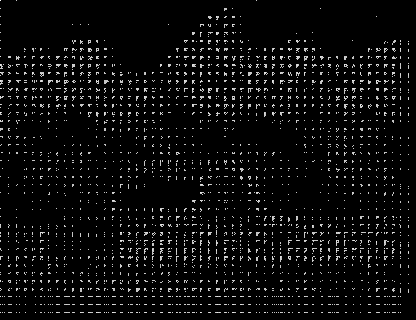
\includegraphics[scale=0.5] {resources/DPCM/Y_DPCM10.png}
                \caption{ Canal Y.}
            \end{subfigure}
            \hfill
            \begin{subfigure}{0.3\textwidth}
                \centering 
                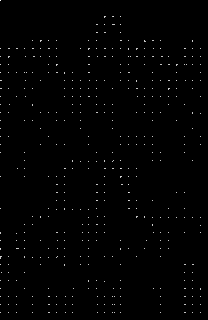
\includegraphics[scale=0.5]{resources/DPCM/CB_DPCM10.png}
                \caption{ Canal Cb.}
            \end{subfigure}
            \hfill
            \begin{subfigure}{0.3\textwidth}
                \centering
                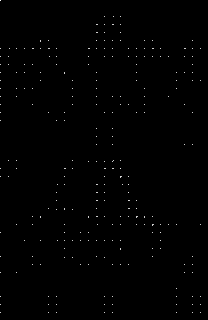
\includegraphics[scale=0.5]{resources/DPCM/CR_DPCM10.png} 
                \caption{ Canal Cr.}
            \end{subfigure}
            \caption{\label{fig:my_label} DPCM da imagem Barn\_Mountains qualidade 10.}
        \end{figure}
        \begin{figure}[H]
            \begin{subfigure}{0.3\textwidth}
                \centering
                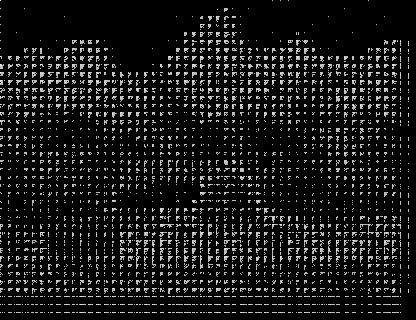
\includegraphics[scale=0.5] {resources/DPCM/Y_DPCM25.png}
                \caption{ Canal Y.}
            \end{subfigure}
            \hfill
            \begin{subfigure}{0.3\textwidth}
                \centering 
                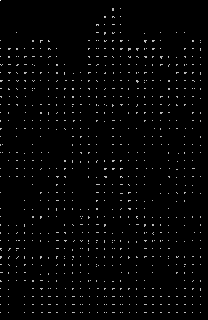
\includegraphics[scale=0.5]{resources/DPCM/CB_DPCM25.png}
                \caption{ Canal Cb.}
            \end{subfigure}
            \hfill
            \begin{subfigure}{0.3\textwidth}
                \centering
                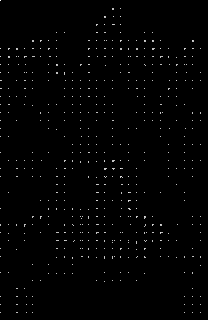
\includegraphics[scale=0.5]{resources/DPCM/CR_DPCM25.png} 
                \caption{ Canal Cr.}
            \end{subfigure}
            \caption{\label{fig:my_label} DPCM da imagem Barn\_Mountains qualidade 25.}
        \end{figure}
        \begin{figure}[H]
            \begin{subfigure}{0.3\textwidth}
                \centering
                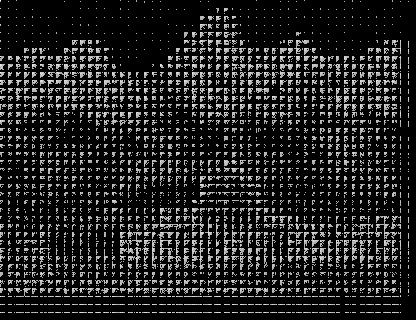
\includegraphics[scale=0.5] {resources/DPCM/Y_DPCM50.png}
                \caption{ Canal Y.}
            \end{subfigure}
            \hfill
            \begin{subfigure}{0.3\textwidth}
                \centering 
                \includegraphics[scale=0.5]{resources/DPCM/CB_DPCM50.png}
                \caption{ Canal Cb.}
            \end{subfigure}
            \hfill
            \begin{subfigure}{0.3\textwidth}
                \centering
                \includegraphics[scale=0.5]{resources/DPCM/CR_DPCM50.png} 
                \caption{ Canal Cr.}
            \end{subfigure}
            \caption{\label{fig:my_label} DPCM da imagem Barn\_Mountains qualidade 50.}
        \end{figure}
        \begin{figure}[H]
            \begin{subfigure}{0.3\textwidth}
                \centering
                \includegraphics[scale=0.5] {resources/DPCM/Y_DPCM75.png}
                \caption{ Canal Y.}
            \end{subfigure}
            \hfill
            \begin{subfigure}{0.3\textwidth}
                \centering 
                \includegraphics[scale=0.5]{resources/DPCM/CB_DPCM75.png}
                \caption{ Canal Cb.}
            \end{subfigure}
            \hfill
            \begin{subfigure}{0.3\textwidth}
                \centering
                \includegraphics[scale=0.5]{resources/DPCM/CR_DPCM75.png} 
                \caption{ Canal Cr.}
            \end{subfigure}
            \caption{\label{fig:my_label} DPCM da imagem Barn\_Mountains qualidade 75.}
        \end{figure}
        \begin{figure}[H]
            \begin{subfigure}{0.3\textwidth}
                \centering
                \includegraphics[scale=0.5] {resources/DPCM/Y_DPCM100.png}
                \caption{ Canal Y.}
            \end{subfigure}
            \hfill
            \begin{subfigure}{0.3\textwidth}
                \centering 
                \includegraphics[scale=0.5]{resources/DPCM/CB_DPCM100.png}
                \caption{ Canal Cb.}
            \end{subfigure}
            \hfill
            \begin{subfigure}{0.3\textwidth}
                \centering
                \includegraphics[scale=0.5]{resources/DPCM/CR_DPCM100.png} 
                \caption{ Canal Cr.}
            \end{subfigure}
            \caption{\label{fig:my_label} DPCM da imagem Barn\_Mountains qualidade 100.}
        \end{figure}

        \begin{table}[H]
            \centering
            \addtolength\tabcolsep{20pt}
            \begin{tabular}{||c | c ||} 
                \hline
                Imagens & Tamanho da DCPM \\
                \hline\hline
                Y\_DCT  & 244 \\
                Cb\_DCT & 58  \\
                Cr\_DCT & 43  \\
                \hline
            \end{tabular}
            \caption{\label{demo-table} Tamanho da DCPM em Kb.}
        \end{table}
    Ao olhar para os resultados da DPCM podemos notar as imagens mais escuras, com menos pontos pontos brancos do que as imagens resultantes da quantização. Isto acontece pelo facto de que na fase de DPCM os coeficientes DC de cada bloco são codificados como a diferença face ao DC do bloco anterior, à excessão do primeiro bloco de todos que se mantém igual. Os coeficientes DC vão ter valores mais baixos e a diferença relativamente aos coeficientes AC diminui, podendo estes ser codificados com menos bits e assim os pontos brancos diminuem.
    
    Em imagens suaves com poucas transições de cor e luz a DPCM obtém melhores resultados uma vez que os coeficientes DC dos vários blocos apresentam valores mais semelhantes.

    \pagebreak
    \section{Imagens descodificadas e erros}
        \begin{multicols}{2}
            \begin{figure}[H]
                \includegraphics[width=\linewidth]{resources/DIFFS/Descodification_quality_10.png}
                \caption{\label{fig:my_label} Imagem descodificada com fator de qualidade 10}
            \end{figure}
            \begin{figure}[H]
                \includegraphics[width=\linewidth]{resources/DIFFS/Diff_Image_with_quality_10.png}
                \caption{\label{fig:my_label} Y error com fator de qualidade 10}
            \end{figure}
        \end{multicols}
        \begin{multicols}{2}
            \begin{figure}[H]
                \includegraphics[width=\linewidth]{resources/DIFFS/Descodification_quality_25.png}
                \caption{\label{fig:my_label} Imagem descodificada com fator de qualidade 25}
            \end{figure}
            \begin{figure}[H]
                \includegraphics[width=\linewidth]{resources/DIFFS/Diff_Image_with_quality_25.png}
                \caption{\label{fig:my_label} Y error com fator de qualidade 25}
            \end{figure}
        \end{multicols}
        \begin{multicols}{2}
            \begin{figure}[H]
                \includegraphics[width=\linewidth]{resources/DIFFS/Descodification_quality_50.png}
                \caption{\label{fig:my_label} Imagem descodificada com fator de qualidade 50}
            \end{figure}
            \begin{figure}[H]
                \includegraphics[width=\linewidth]{resources/DIFFS/Diff_Image_with_quality_50.png}
                \caption{\label{fig:my_label} Y error com fator de qualidade 50}
            \end{figure}
        \end{multicols}
        \pagebreak
        \begin{multicols}{2}
            \begin{figure}[H]
                \includegraphics[width=\linewidth]{resources/DIFFS/Descodification_quality_75.png}
                \caption{\label{fig:my_label} Imagem descodificada com fator de qualidade 75}
            \end{figure}
            \begin{figure}[H]
                \includegraphics[width=\linewidth]{resources/DIFFS/Diff_Image_with_quality_75.png}
                \caption{\label{fig:my_label} Y error com fator de qualidade 75}
            \end{figure}
        \end{multicols}
        \begin{multicols}{2}
            \begin{figure}[H]
                \includegraphics[width=\linewidth]{resources/DIFFS/Descodification_quality_100.png}
                \caption{\label{fig:my_label} Imagem descodificada com fator de qualidade 100}
            \end{figure}
            \begin{figure}[H]
                \includegraphics[width=\linewidth]{resources/DIFFS/Diff_Image_with_quality_100.png}
                \caption{\label{fig:my_label} Y error com fator de qualidade 100}
            \end{figure}
        \end{multicols}

    Nas figuras acima temos representadas as diferenças
entre o canal Y de cada uma das imagens originais e da imagem descodificada
respetiva (erro), para cada um dos fatores de qualidade testados.
Quanto menor o fator de qualidade mais marcadas \footnote{
Subentendemos \emph{marcadas} como a semelhança que a imagem do erro tem com a imagem original. Uma imagem mais \emph{marcada} significa que se assemelha mais à imagem original.
}
estão as imagens (estas marcas são maiores e mais visíveis quanto maior for a compressão ocorrida nessa área), o que era esperado uma vez que quanto menor é o fator, maior é a compressão e perda de informação, resultando num erro maior.

\section{Métricas de distorção}

Calculamos, para cada imagem com cada fator de qualidade, métricas de distorção que permitem analisar e comparar as diferenças entre a imagem original e as imagens reconstruidas. 
Fizemos o calculo do MSE (Mean squared error) que mede a diferença média ao quadrado entre os pixeis das duas imagens e o RMSE (Root Mean Square Error) que é a raiz quadrada do anterior. Quanto maiores são estes valores maior a diferença entre as duas imagens, ou seja, maiores as perdas de informação.

Obtemos também o SNR (Signal-to-noise ratio) que mede a razão entre a amplitude do sinal e a amplitude do ruído na imagem, e o PSNR (Peak signal-to-noise ratio) que é a razão entre a potência máxima possível de um sinal e a potência do ruído presente. Maiores valores destas duas métricas indicam melhor qualidade na imagem (menos ruído), 
Por fim calculamos a média do Y error representados nas imagens acima. 

    \begin{table}[H]
            \centering
            %\addtolength\tabcolsep{15pt}
            \begin{tabular}{||c | c c c c c||} 
                \hline
                barn\_mountains & 10 & 25 & 50 & 75 & 100 \\ 
                \hline\hline
                MSE &  709.672 &  399.375 & 261.932 & 152.652 & 8.942 \\
                RMSE & 26.639 &  19.984 &   16.184  & 12.355  & 2.990 \\
                SNR &  18.675 &  21.172 &  23.004  & 25.349  & 37.671 \\
                PSNR & 19.620 &  22.116 &   23.948 & 26.293  & 38.616\\
                Mean &  9.452 &  6.778 &  5.268  &  3.844 & 0.211 \\
                \hline
            \end{tabular}
            \caption{\label{demo-table} Metricas de distorção da imagem barn-mountains.bmp}
        \end{table}

    \begin{table}[H]
            \centering
            %\addtolength\tabcolsep{15pt}
            \begin{tabular}{||c | c c c c c||} 
                \hline
                logo & 10 & 25 & 50 & 75 & 100 \\ 
                \hline\hline
                MSE &  158.921 &  66.608  & 43.168 & 22.943 &   4.520 \\
                RMSE &   12.606 &   8.161  &  6.570 &  4.789 &  2.126 \\
                SNR &   29.320  &  33.096  & 34.980 & 37.725 & 44.780 \\
                PSNR &   26.118 &   29.895 &  31.779&  34.524 & 41.578\\
                Mean &  5.211 &  1.520 &  1.275  &  0.445 & 0.038 \\
                \hline
            \end{tabular}
            \caption{\label{demo-table} Metricas de distorção da imagem logo.bmp}
        \end{table}

    \begin{table}[H]
            \centering
            %\addtolength\tabcolsep{15pt}
            \begin{tabular}{||c | c c c c c||} 
                \hline
                peppers & 10 & 25 & 50 & 75 & 100 \\ 
                \hline\hline
                MSE &    287.667 &  129.383  & 77.917 & 50.335 &   4.981 \\
                RMSE &   16.960 &   11.374  &  8.827 &  7.094 &  2.231 \\
                SNR &    20.337  &  23.807  & 26.009 & 27.907 & 37.952 \\
                PSNR &   23.541 &   27.012 &  29.214 & 31.112 & 41.157\\
                Mean &  4.487 &  2.680  &  1.965  & 1.483  & 0.230 \\
                \hline
            \end{tabular}
            \caption{\label{demo-table} Metricas de distorção da imagem peppers.bmp}
        \end{table}

    Da analise dos resultados obtivemos, para todas as imagens, valores esperados consoante a descrição de cada métrica. Os valores de MSE e RMSE foram decrescendo com o aumento do fator de qualidade, uma vez que as diferenças das imagens descodificadas com as originais vão sendo menores. Já os valores de SNR e PSNR foram aumentando com o aumento do fator de qualidade devido ao facto do ruído progressivamente decrescer. Por fim os valores da média das diferenças entre os canais Y das imagens originais e descodificadas foi decrescendo com o aumento do fator de qualidade, como era também esperado.
    
\pagebreak
\section{Conclusão}
    No final deste trabalho conseguimos adquirir o conhecimento impirico sobre o funcionamento do JPEG:
    \begin{itemize}
        \item Permite fazer compressões nas imagens de alta resolução;
        \item Imagens de cores sólidas e transições suaves irão ter alta compressão;
        \item Imagens com transições de cores abruptas podem resultar em perdas de qualidade e detalhe mais acentuadas;
    \end{itemize}

\end{document}
